\chapter{Priorit\"ats-Warteschlangen \label{chap:prioqueue}}
Um den Begriff der  \emph{Priorit\"ats-Warteschlange} zu verstehen, betrachten wir zun\"achst
den Begriff der \emph{Warteschlange}.  Dort werden Daten hinten eingef\"ugt und vorne werden
Daten entnommen. Das f\"uhrt dazu, dass Daten in derselben Reihenfolge entnommen werden,
wie sie eingef\"ugt werden.  Anschaulich ist das so wie bei der Warteschlange vor einer
Kino-Kasse, wo die Leute in der Reihenfolge bedient werden, in der sie sich anstellen.
Bei einer Priorit\"ats-Warteschlange haben die Daten zus\"atzlich Priorit\"aten.  Es wird immer
das Datum entnommen, was die h\"ochste Priorit\"at hat.  Anschaulich ist das so wie im
Wartezimmer eines Zahnarztes. Wenn Sie schon eine Stunde gewartet haben und dann ein
Privat-Patient aufkreuzt, dann m\"ussen Sie halt noch eine Stunde warten, weil der
Privat-Patient eine h\"ohere Priorit\"at hat.

Priorit\"ats-Warteschlangen spielen in vielen Bereichen der Informatik  eine wichtige
Rolle.  Wir werden Priorit\"ats-Warteschlangen sp\"ater sowohl in dem Kapitel \"uber
Daten-Kompression als auch bei der Implementierung des Algorithmus zur Bestimmung
k\"urzester Wege in einem Graphen einsetzen.  Daneben werden Priorit\"ats-Warteschlangen unter anderem in
Simulations-Systemen und beim Scheduling von Prozessen in Betriebs-Systemen eingesetzt.


\section{Definition des ADT \textsl{PrioQueue}}
Wir versuchen den Begriff der Priorit\"ats-Warteschlange jetzt formal durch Definition eines
abstrakten Daten-Typs zu fassen.
Wir geben hier eine eingeschr\"ankte Definition von Priorit\"ats-Warteschlangen, die nur die
Funktionen enth\"alt, die wir sp\"ater f\"ur den Algorithmus von Dijkstra ben\"otigen.
\begin{Definition}[Priorit\"ats-Warteschlange] \hspace*{\fill} \\
{\em
  Wir definieren den abstrakten Daten-Typ der \emph{Priorit\"ats-Warteschlange} wie folgt:
  \begin{enumerate}
  \item Als Namen w\"ahlen wir \textsl{PrioQueue}.
  \item Die Menge der Typ-Parameter ist \\[0.1cm]
        \hspace*{1.3cm} $\{ \textsl{Key}, \textsl{Value} \}$.

        Dabei muss auf der Menge $\textsl{Key}$ eine totale Quasi-Ordnung $<$ existieren,
        so dass wir die Priorit\"aten verschiedener Elemente anhand der Schl\"ussel
        vergleichen k\"onnen. 
  \item Die Menge der Funktions-Zeichen ist \\[0.1cm]
       \hspace*{1.3cm} 
       $\{ \textsl{PrioQueue}, \textsl{insert}, \textsl{remove}, \textsl{top}, \textsl{change} \}$.
  \item Die Typ-Spezifikationen der Funktions-Zeichen sind gegeben durch:
        \begin{enumerate}
        \item $\textsl{PrioQueue}: \textsl{PrioQueue}$

              Der Aufruf ``$\textsl{PrioQueue}()$'' erzeugt eine leere
              Priorit\"ats-Warteschlange. 
        \item $\textsl{top}: \textsl{PrioQueue}  \rightarrow (\textsl{Key} \times \textsl{Value}) \cup \{\Omega\}$

              Der Aufruf $Q.\textsl{top}()$ liefert ein Paar $\pair(k,v)$.  Dabei ist $v$ ein Element
              aus $Q$, das eine maximale Priorit\"at hat. $k$ ist die Priorit\"at des Elements $v$.
        \item $\textsl{insert}: \textsl{PrioQueue} \times \textsl{Key} \times \textsl{Value} \rightarrow \textsl{PrioQueue}$

              Der Aufruf $Q.\textsl{insert}(k,v)$ f\"ugt das Element $v$ mit der Priorit\"at $k$ in
              die Priorit\"ats-Warteschlange $Q$ ein.  
        \item $\textsl{remove}: \textsl{PrioQueue} \rightarrow \textsl{PrioQueue}$

              Der Aufruf $Q.\textsl{remove}()$ entfernt aus der Priorit\"ats-Warteschlange
              $Q$ ein Element, das eine maximale Priorit\"at hat.
        \item $\textsl{change}: \textsl{PrioQueue} \times \textsl{Key} \times \textsl{Value} \rightarrow \textsl{PrioQueue}$

              Der Aufruf $Q.\textsl{change}(k,v)$ \"andert die Priorit\"at des Elements $v$ in
              der Priorit\"ats-Warte\-schlange $Q$ so ab, dass
              $k$ die neue Priorit\"at dieses Elements ist. 
              Wir setzen dabei voraus, dass einerseits dass Element $v$ in der
              Priorit\"ats-Warteschlange $Q$ auftritt und dass andererseits die neue
              Priorit\"at mindestens so hoch ist wie die Priorit\"at, die $v$
              vorher hatte.
        \end{enumerate}
\item Bevor wir das Verhalten der einzelnen Methoden axiomatisch definieren, m\"ussen wir
      noch festlegen, was wir unter den \emph{Priorit\"aten} verstehen wollen, die den
      einzelnen Elementen aus $\textsl{Value}$ zugeordnet sind.  Wir nehmen an, dass die
      Priorit\"aten Elemente einer Menge $\textsl{Key}$ sind und dass auf der Menge \textsl{Key}
      eine totale Quasi-Ordnung $\leq$ existiert. Falls dann $k_1 < k_2$ ist, sagen wir, 
      dass $k_1$ eine h\"ohere Priorit\"at als $k_2$ hat.  Dass die Priorit\"aten h\"oher
      werden wenn die Schl\"ussel kleiner werden erscheint im ersten Moment vielleicht
      paradox. Es wird aber sp\"ater verst\"andlich, wenn wir den Algorithmus zur
      Berechnung k\"urzester Wege von Dijkstra diskutieren. Dort sind die Priorit\"aten
      Entfernungen im Graphen und die Priorit\"at eines Knotens ist um so h\"oher, je n\"aher
      der Knoten zu einem als \emph{Startknoten} ausgezeichneten Knoten ist. 

      Wir spezifizieren das Verhalten der Methoden nun dadurch, dass wir eine einfache
      \emph{Referenz-Implementierung} des ADT \textsl{PrioQueue} angeben und dann fordern,
      dass sich eine Implementierung des ADT \textsl{PrioQueue} genauso verh\"alt wie unsere
      Referenz-Implementierung.  Bei unserer Referenz-Implementierung stellen wir eine
      Priorit\"ats-Warteschlange durch eine Menge von Paaren von Priorit\"aten und Werten 
      dar.   F\"ur solche Mengen definieren wir unserer Methoden wie folgt.
      \begin{enumerate}
      \item $\textsl{PrioQueue}() = \{\}$,

             der Konstruktor erzeugt also eine leere
            Priorit\"ats-Warteschlange, die als leere Menge dargestellt wird. 
      \item $Q.\textsl{insert}(k, v) = Q \cup \{ \pair(k,v) \}$,
        
            Um einen Wert $v$ mit einer Priorit\"at $k$ in die Priorit\"ats-Warteschlange 
            $Q$ einzuf\"ugen, reicht es aus, das Paar $\pair(k,v)$ zu der Menge $Q$ hinzuzuf\"ugen.
      \item Wenn $Q$ leer ist, dann ist $Q.\textsl{top}()$ undefiniert: \\[0.1cm]
            \hspace*{1.3cm} $Q = \{\} \;\rightarrow\; Q.\textsl{top}() = \Omega$.
     \item Wenn $Q$ nicht leer ist, wenn es also ein Paar $\pair(k_1, v_1)$ in $Q$
              gibt, dann liefert $Q.\textsl{top}()$ ein Paar $\pair(k_2,v)$ aus der Menge
              $Q$, so dass der Schl\"ussel $k_2$ minimal wird.  Dann gilt also f\"ur
              alle $\pair(k_1,v_1) \in Q$, dass $k_2 \leq k_1$ ist.  Formal k\"onnen wir schreiben:
              \\[0.1cm]
              \hspace*{1.3cm} 
              $\pair(k_1,v_1) \in Q \;\wedge\; Q.\textsl{top}() = \pair(k_2,v_2)
              \;\rightarrow\; k_2 \leq k_1 \;\wedge\; \pair(k_2,v_2) \in Q$.
      \item Falls $Q$ leer ist, dann \"andert $\textsl{remove}()$ nichts daran: \\[0.1cm]
            \hspace*{1.3cm} $Q = \{\} \rightarrow Q.\textsl{remove}() = Q$.
      \item Sonst entfernt $Q.\textsl{remove}()$ ein Paar mit der h\"ochsten Priorit\"at: \\[0.1cm]
            \hspace*{1.3cm} 
            $Q \not= \{\} \rightarrow Q.\textsl{remove}() = Q \backslash \bigl\{ Q.\textsl{top}() \bigr\}$.
      \item Die Methode \textsl{change}() \"andert die Priorit\"at des Paares,
            dessen Wert als Argument \"ubergeben wird: \\[0.1cm]
            \hspace*{1.3cm} 
            $Q.\textsl{change}(k_1,v_1) = \bigl\{ \pair(k_2,v_2) \in Q \mid v_2 \not= v_1 \bigr\} \cup \bigl\{ \pair(k_1,v_1) \bigr\}$.
      \end{enumerate}
\end{enumerate}
}
\end{Definition}

Wir k\"onnen den abstrakten Daten-Typ \textsl{PrioQueue} dadurch implementieren,
dass wir eine Priorit\"ats-Warteschlange durch eine Liste realisieren, in der die Elemente
aufsteigend geordnet sind. Die einzelnen Operationen werden dann wie folgt implementiert:
\begin{enumerate}
\item $\textsl{PrioQueue}()$ erzeugt eine leere Liste.
\item $Q.\textsl{insert}(d)$ kann durch die Prozedur \texttt{insert} implementiert werden,
      die wir beim ``\emph{Sortieren durch Einf\"ugen}'' entwickelt haben.
\item $Q.\textsl{top}()$ gibt das erste Element der Liste zur\"uck.
\item $Q.\textsl{remove}()$ entfernt das erste Element der Liste.
\item $Q.\textsl{change}(k,v)$ geht alle Eintr\"age der Liste durch.
      Falls dabei ein Eintrag mit dem Wert $v$ gefunden wird, so wird das zugeh\"orige
      Paar aus der Liste gel\"oscht.  Anschlie\3end wird das Paar $\pair(k,v)$ neu in die
      Liste eingef\"ugt.
\end{enumerate}
Bei dieser Implementierung ist die Komplexit\"at der Operationen $\textsl{insert}()$ und
$\textsl{change}()$ linear in der
Anzahl $n$ der Elemente der Priorit\"ats-Warteschlange.  Alle anderen Operationen sind
konstant. Wir werden jetzt eine andere
Implementierung vorstellen, bei der die Komplexit\"at von $\textsl{insert}()$ und
$\textsl{change}()$ den Wert $\Oh\bigl(\log(n)\bigr)$ hat.  Dazu m\"ussen wir eine neue Daten-Struktur einf\"uhren: \emph{Heaps}.

\section{Die Daten-Struktur \emph{Heap}}
Wir definieren die Menge \textsl{Heap}\footnote{
Der Begriff \textsl{Heap} wird in der Informatik f\"ur zwei unterschiedliche Dinge
verwendet:  Zum einen wird die in diesem Abschnitt beschriebene Daten-Struktur als
\textsl{Heap} bezeichnet, zum anderen wird der Teil des Speichers, in dem dynamisch
erzeugte Objekte abgelegt werden, als \textsl{Heap} bezeichnet.}
induktiv als Teilmenge der Menge $\Bin$ der
bin\"aren B\"aume. Dazu definieren wir zun\"achst f\"ur einen Schl\"ussel $k_1\in \textsl{Key}$ und
einen bin\"aren Baum $b \in \Bin$ die Relation $k_1 \leq b$ durch Induktion \"uber $b$.
Die Intention ist dabei, dass $k_1 \leq b$ genau dann gilt, wenn f\"ur jeden Schl\"ussel $k_2$,
der in $b$ auftritt,  $k_1 \leq k_2$ gilt. Die formale Definition ist wie folgt:
\begin{enumerate}
\item $k_1 \leq \textsl{nil}$,

      denn in dem leeren Baum treten \"uberhaupt keine Schl\"ussel auf.
\item $k_1 \leq \textsl{node}(k_2,v,l,r) \;\stackrel{\mbox{\scriptsize def}}{\longleftrightarrow}\; k_1 \leq k_2 \;\wedge\; k_1 \leq l \;\wedge\; k_1 \leq r$,
         
      denn $k_1$ ist genau dann kleiner-gleich als alle Schl\"ussel, die in dem Baum 
      $\textsl{node}(k_2,v,l,r)$ auftreten, wenn $k_1 \leq k_2$ gilt und wenn zus\"atzlich
      $k_1$ kleiner-gleich als alle Schl\"ussel ist, die in $l$ oder $r$ auftreten.
\end{enumerate}
Als n\"achstes definieren wir eine Funktion \\[0.1cm]
\hspace*{1.3cm} $\textsl{count}: \Bin \rightarrow \mathbb{N}$, \\[0.1cm]
die f\"ur einen bin\"aren Baum die Anzahl der Knoten berechnet.  Die Definition erfolgt durch
Induktion:
\begin{enumerate}
\item $\textsl{nil}.\textsl{count}() = 0$.
\item $\textsl{node}(k,v,l,r).\textsl{count}() = 1 + l.\textsl{count}() + r.\textsl{count}()$.
\end{enumerate}
Mit diesen Vorbereitungen k\"onnen wir nun die Menge \textsl{Heap} induktiv definieren:
\begin{enumerate}
\item $\textsl{nil} \in \textsl{Heap}$.
\item $\textsl{node}(k,v,l,r) \in \textsl{Heap}$ g.d.w. folgendes gilt:
      \begin{enumerate}
      \item $k \leq l \;\wedge\; k \leq r$,

            Der Schl\"ussel an der Wurzel ist also kleiner-gleich als alle anderen Schl\"ussel.
            Diese Bedingung bezeichnen wir auch als die \emph{Heap-Bedingung}.
      \item $\mid l.\textsl{count}() - r.\textsl{count}() \mid \;\leq\, 1$,

            Die Zahl der Schl\"ussel im linken Teilbaum ist also h\"ochstens 1 gr\"o\3er oder
            kleiner als die Zahl der Schl\"ussel im rechten Teilbaum.
            Diese Bedingung bezeichen wir als die \emph{Balancierungs-Bedingung}.  Sie ist
            ganz \"ahnlich zu der Balancierungs-Bedingung bei AVL-B\"aumen, nur dass es dort
            die H\"ohe der B\"aume ist, die verglichen wird, w\"ahrend wir hier die Zahl der
            im Baum gespeicherten Elemente vergleichen.
      \item $l \in \textsl{Heap} \;\wedge\; r \in \textsl{Heap}$.
      \end{enumerate}
\end{enumerate}
Aus der \emph{Heap-Bedingung} folgt, dass ein nicht-leerer Heap die Eigenschaft hat, dass
das Element, welches an der Wurzel steht, immer die h\"ochste Priorit\"at hat.  Abbildung
\ref{fig:heap-list} auf Seite \pageref{fig:heap-list} zeigt einen einfachen Heap.
In den Knoten steht im oberen Teil die Priorit\"aten (in der Abbildung sind das nat\"urliche Zahlen) und
darunter stehen die Werte (in der Abbildung sind dies Buchstaben).

\begin{figure}[!t]
  \centering
  \framebox{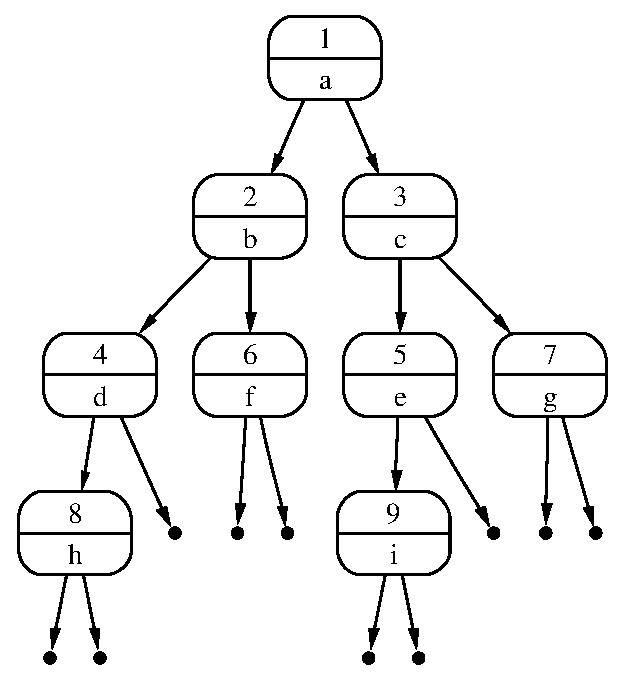
\epsfig{file=heap-with-holes,scale=0.7}} 
  \caption{Ein Heap}
  \label{fig:heap-list}
\end{figure}


Da Heaps bin\"are
B\"aume sind, k\"onnen wir Sie ganz \"ahnlich wie geordnete bin\"are B\"aume  implementieren. 
Wir stellen zun\"achst Gleichungen auf, die die Implementierung der verschiedenen Methoden
beschreiben.  Wir beginnen mit der  Methode \textsl{top}.  Es gilt:
\begin{enumerate}
\item $\textsl{nil}.\textsl{top}() = \Omega$.
\item $\textsl{node}(k,v,l,r).\textsl{top}() = \pair(k,v)$,

      denn aufgrund der Heap-Bedingung wird der Wert mit der h\"ochsten Priorit\"at 
      an der Wurzel gespeichert.
\end{enumerate}
Die Methoden \textsl{insert} m\"ussen wir nun so implementieren, dass
sowohl die Balancierungs-Bedingung als auch die Heap-Bedingung erhalten bleiben.
\begin{enumerate}
\item $\textsl{nil}.\textsl{insert}(k,v) = \textsl{node}(k,v,\textsl{nil}, \textsl{nil})$.
\item $k_{\mathrm{top}} \leq k \;\wedge\; l.\textsl{count}() \leq r.\textsl{count}() \;\rightarrow $   \\[0.1cm]
      \hspace*{1.3cm} 
      $\textsl{node}(k_{\mathrm{top}},v_\mathrm{top},l,r).\textsl{insert}(k,v) =
                 \textsl{node}\bigl(k_\mathrm{top},v_\mathrm{top},l.\textsl{insert}(k,v), r\bigr)$.

      Falls das einzuf\"ugende Paar eine geringere oder dieselbe Priorit\"at hat wie das
      Paar, welches sich an der Wurzel befindet, und falls zus\"atzlich die Zahl der Paare im linken Teilbaum
      kleiner-gleich der Zahl der Paare im rechten Teilbaum ist, dann f\"ugen wir das
      Paar im linken Teilbaum ein.
\item $k_{\mathrm{top}} \leq k \;\wedge\; l.\textsl{count}() > r.\textsl{count}() \;\rightarrow $   \\[0.1cm]
      \hspace*{1.3cm} 
      $\textsl{node}(k_{\mathrm{top}},v_\mathrm{top},l,r).\textsl{insert}(k,v) =
                 \textsl{node}\bigl(k_\mathrm{top},v_\mathrm{top},l,r.\textsl{insert}(k,v)\bigr)$.

      Falls das einzuf\"ugende Paar eine geringere oder dieselbe Priorit\"at hat als das
      Paar an der Wurzel und falls zus\"atzlich die Zahl der Paare im linken Teilbaum
      gr\"o\3er als die Zahl der Paare im rechten Teilbaum ist, dann f\"ugen wir das
      Paar im rechten Teilbaum ein.
\item $k_{\mathrm{top}} > k \;\wedge\; l.\textsl{count}() \leq r.\textsl{count}() \;\rightarrow $ \\[0.1cm]
      \hspace*{1.3cm} 
      $\textsl{node}(k_{\mathrm{top}},v_\mathrm{top},l,r).\textsl{insert}(k,v) =
                 \textsl{node}\bigl(k,v,l.\textsl{insert}(k_\mathrm{top},v_\mathrm{top}), r\bigr)$.

      Falls das einzuf\"ugende Paar eine h\"ohere Priorit\"at hat als das Paar an
      der Wurzel, dann m\"ussen wir das neu einzuf\"ugende Paar an der Wurzel
      positionieren.  Das Paar, das dort vorher steht, f\"ugen wir in den linken
      Teilbaum ein, falls  die Zahl der Paare im linken Teilbaum
      kleiner-gleich der Zahl der Paare im rechten Teilbaum ist.
\item $k_{\mathrm{top}} > k \;\wedge\; l.\textsl{count}() > r.\textsl{count}() \;\rightarrow $ \\[0.1cm] 
      \hspace*{1.3cm} 
      $\textsl{node}(k_{\mathrm{top}},v_\mathrm{top},l,r).\textsl{insert}(k,v) =
                 \textsl{node}\bigl(k,v,l,r.\textsl{insert}(k_\mathrm{top},v_\mathrm{top})\bigr)$.

      Falls wir das einzuf\"ugende Paar an der Wurzel
      positionieren m\"ussen und die Zahl der Paare im linken Teilbaum
      gr\"o\3er als die Zahl der Paare im rechten Teilbaum ist,
      dann m\"ussen wir das Paar, das vorher an der Wurzel stand, im rechten Teilbaum
      einf\"ugen.
\end{enumerate}
Als n\"achstes beschreiben wir die Implementierung der Methode \textsl{remove}.
\begin{enumerate}
\item $\textsl{nil}.\textsl{remove}() = \textsl{nil}$,

      denn aus dem leeren Heap ist nichts mehr zu entfernen.
\item $\textsl{node}(k,v,\textsl{nil},r).\textsl{remove}() = r$,
  
\item $\textsl{node}(k,v,l,\textsl{nil}).\textsl{remove}() = l$,

      denn wir entfernen immer das Paar mit der h\"ochsten Priorit\"at und das ist an der
      Wurzel.  Wenn einer der beiden Teilb\"aume leer ist, k\"onnen wir einfach den anderen
      zur\"uck geben.

      Jetzt betrachten wir die F\"alle, wo keiner der beiden Teilb\"aume leer ist.
      Dann muss entweder das Paar an der Wurzel des linken Teilbaums
      oder das Paar an der Wurzel des rechten Teilbaums an die Wurzel aufr\"ucken.
      Welches dieser beiden Paare wir nehmen, h\"angt davon ab, welches dr Paare die h\"ohere
      Priorit\"at hat.
\item $k_1 \leq k_2 \;\wedge\; l = \textsl{node}(k_1,v_1,l_1,r_1) \;\wedge\; r =
      \textsl{node}(k_2,v_2,l_2,r_2) \;\rightarrow$ \\[0.1cm] 
      \hspace*{1.3cm} 
      $\textsl{node}(k,v,l,r).\textsl{remove}() =      \textsl{node}(k_1,v_1,l.\textsl{remove}(),r)$,

      denn wenn das Paar an der Wurzel des linken Teilbaums eine h\"ohere Priorit\"at hat
      als das Paar an der Wurzel des rechten Teilbaums, dann r\"uckt dieses Paar an
      die Wurzel auf und muss folglich aus dem linken Teilbaum gel\"oscht werden.
\item $k_1 > k_2 \;\wedge\; l = \textsl{node}(k_1,v_1,l_1,r_1) \;\wedge\; r = \textsl{node}(k_2,v_2,l_2,r_2) \rightarrow$ \\[0.1cm]
      \hspace*{1.3cm} 
      $\textsl{node}(k,v,l,r).\textsl{remove}() = \textsl{node}(k_2,v_2,l,r.\textsl{remove}())$,

      denn wenn das Paar an der Wurzel des rechten Teilbaums eine h\"ohere Priorit\"at hat
      als das Paar an der Wurzel des linken Teilbaums, dann r\"uckt dieses Paar an
      die Wurzel auf und muss folglich aus dem rechten Teilbaum gel\"oscht werden.  
\end{enumerate}
An dieser Stelle wird der aufmerksame Leser vermutlich bemerken, dass die obige
Implementierung der Methode \textsl{remove} die Balancierungs-Bedingung verletzt.
Es ist nicht schwierig, die Implementierung so abzu\"andern, dass die
Balancierungs-Bedingung erhalten bleibt. Es zeigt sich jedoch, dass die
Balancierungs-Bedingung  nur beim Aufbau eines Heaps mittels \textsl{insert}() wichtig ist,
denn dort garantiert sie, dass die H\"ohe des Baums in logarithmischer Weise von der Zahl
seiner Knoten abh\"angt.  Beim L\"oschen wird die H\"ohe des Baums sowieso nur kleiner, also
brauchen wir uns da keine Sorgen machen.

\section{Implementierung in \textsl{Java}}

\begin{figure}[!h]
  \centering
\begin{Verbatim}[ frame         = lines, 
                  framesep      = 0.3cm, 
                  labelposition = bottomline,
                  numbers       = left,
                  numbersep     = -0.2cm,
                  xleftmargin   = 0.0cm,
                  xrightmargin  = 0.0cm
                ]
    public abstract class HeapNode<Key extends Comparable<Key>, Value>
    {
        protected int mCount;
    
        public abstract Pair<Key, Value> top();
        public abstract BinaryHeapNode<Key, Value> insert(Key key, Value value);
        public abstract HeapNode<Key, Value> remove();    
        public abstract boolean isEmpty();
    }
\end{Verbatim}
\vspace*{-0.3cm}
  \caption{Die abstrakte Klasse \textsl{HeapNode}.}
  \label{fig:HeapNode}
\end{figure}
Zun\"achst implementieren wir eine abstrakte Klasse \textsl{HeapNode}.  Elemente dieser
Klasse sollen Heaps repr\"asentieren und zwar sowohl leere Heaps als auch nicht-leere Heaps.
Abbildung \ref{fig:HeapNode} auf Seite \pageref{fig:HeapNode} zeigt die Implementierung.
Wir haben eine Member-Variable mit dem Namen \texttt{mCount} in Zeile 3 definiert.
Diese Variable gibt die Zahl der in dem Heap abgespeicherten Werte an.

Wir werden uns mit der Implementierung der Methode $\textsl{change}()$ erst sp\"ater
besch\"aftigen. Daher fehlt diese Methode in der Klasse \textsl{HeapNode}.
Statt dessen haben wir eine zus\"atzliche Methode \textsl{isEmpty}(), die wir sp\"ater bei der
Implementierung der Methoden \textsl{insert}() und \textsl{remove}() benutzen werden.

\begin{figure}[!h]
  \centering
\begin{Verbatim}[ frame         = lines, 
                  framesep      = 0.3cm, 
                  labelposition = bottomline,
                  numbers       = left,
                  numbersep     = -0.2cm,
                  xleftmargin   = 0.0cm,
                  xrightmargin  = 0.0cm
                ]
    public class EmptyHeapNode<Key extends Comparable<Key>, Value> 
        extends HeapNode<Key, Value>
    {
        public EmptyHeapNode() {
            mCount = 0;
        }    
        public Pair<Key, Value> top() {
            return null;
        }
        public BinaryHeapNode<Key, Value> insert(Key key, Value value) {
            return new BinaryHeapNode<Key, Value>(key, value);
        }        
        public HeapNode<Key, Value> remove() {
            return this;
        }
        public boolean isEmpty() {
            return true;
        }
    }
\end{Verbatim}
\vspace*{-0.3cm}
  \caption{Die Klasse \textsl{EmptyHeapNode}.}
  \label{fig:EmptyHeapNode}
\end{figure}

Abbildung \ref{fig:EmptyHeapNode} auf Seite \pageref{fig:EmptyHeapNode} zeigt die
Implementierung der Klasse \textsl{EmptyHeapNode}.  Elemente dieser Klasse repr\"asentieren
den leeren Heap \textsl{nil}.  Im Konstruktor setzen wir in Zeile 5 die Member-Variable
\texttt{mCount} auf 0, denn der leere Heap enth\"alt keine Werte. Die Methode \textsl{top}()
gibt \texttt{null} zur\"uck, denn es gibt ja keinen sinnvollen Wert, den wir hier zur\"uck
geben k\"onnen.   Die Methode \textsl{insert}() erzeugt einen neuen Knoten vom Typ
\textsl{BinaryHeapNode}, der dann zur\"uck gegeben wird. 


\begin{figure}[!h]
  \centering
\begin{Verbatim}[ frame         = lines, 
                  framesep      = 0.3cm, 
                  labelposition = bottomline,
                  numbers       = left,
                  numbersep     = -0.2cm,
                  xleftmargin   = 0.0cm,
                  xrightmargin  = 0.0cm
                ]
    public class BinaryHeapNode<Key extends Comparable<Key>, Value> 
        extends HeapNode<Key, Value>
    {
        private Key                  mKey;    // The priority associated with the value.
        private Value                mValue;  // The value.
        private HeapNode<Key, Value> mLeft;   // The root of the left subtree.
        private HeapNode<Key, Value> mRight;  // The root of the right subtree.
    
        public BinaryHeapNode(Key key, Value value) {
            mKey    = key;
            mValue  = value;
            mLeft   = new EmptyHeapNode<Key, Value>();
            mRight  = new EmptyHeapNode<Key, Value>();
            mCount  = 1;
        }    
        public Pair<Key, Value> top() {
            return new Pair<Key, Value>(mKey, mValue);
        }
        public BinaryHeapNode<Key, Value> insert(Key key, Value value)
        {
            ++mCount;
            int cmp = key.compareTo(mKey);
            if (cmp < 0) {                         
                if (mLeft.mCount > mRight.mCount) {
                    mRight = mRight.insert(mKey, mValue);
                } else {
                    mLeft = mLeft.insert(mKey, mValue);
                }
                mKey   = key;
                mValue = value;
            } else {
                if (mLeft.mCount > mRight.mCount) {
                    mRight = mRight.insert(key, value);
                } else {
                    mLeft = mLeft.insert(key, value);
                }
            }
            return this;
        }        
        public boolean isEmpty() {
            return false;
        }
\end{Verbatim}
\vspace*{-0.3cm}
  \caption{Die Klasse \textsl{BinaryHeapNode}, Teil I.}
  \label{fig:BinaryHeapNode-I}
\end{figure}
Die Klasse \textsl{BinaryHeapNode}, deren Implementierung in den Abbildungen
\ref{fig:BinaryHeapNode-I} und \ref{fig:BinaryHeapNode-II} auf den Seiten
\pageref{fig:BinaryHeapNode-I} und \pageref{fig:BinaryHeapNode-II} gezeigt wird,
repr\"asentiert einen Knoten der Form \\[0.1cm]
\hspace*{1.3cm} 
$\textsl{node}(\texttt{mKey}, \mathtt{mValue}, \mathtt{mLeft}, \mathtt{mRight})$. 
\\[0.1cm]
Die Implementierung setzt die rekursiven Gleichungen, die wir im vorhergehenden
Unterabschnitt gezeigt haben, 1-zu-1 um.  Diskutiert werden muss h\"ochstens noch die
Implementierung der Methode \textsl{remove}.  Wenn der Kontrollfluss in Zeile 51 ankommt,
dann ist klar, dass weder der linke Teilbaum \texttt{mLeft} noch der rechte Teilbaum
\texttt{mRight} leer ist.
Daher sind diese Teilb\"aume Objekte der Klasse \textsl{BinaryHeapNode} und wir k\"onnen
\texttt{mLeft} und \texttt{mRight} auf den Typ \textsl{BinaryHeapNode} casten.
Dies ist notwendig, weil wir auf die Schl\"ussel, die an der Wurzel dieser B\"aume
abgespeichert sind, zur\"uckgreifen m\"ussen.  Das geht aber nur, wenn diese den Typ
\textsl{BinaryHeapNode} haben, denn nur in diesem Typ sind die Member-Variablen
\texttt{mKey} und \texttt{mValue} definiert.

\begin{figure}[!h]
  \centering
\begin{Verbatim}[ frame         = lines, 
                  framesep      = 0.3cm, 
                  firstnumber   = last,
                  labelposition = bottomline,
                  numbers       = left,
                  numbersep     = -0.2cm,
                  xleftmargin   = 0.0cm,
                  xrightmargin  = 0.0cm
                ]
        public HeapNode<Key, Value> remove() {
            --mCount;
            if (mLeft.isEmpty()) {
                return mRight;
            } 
            if (mRight.isEmpty()) {
                return mLeft;
            }
            BinaryHeapNode<Key, Value> left  = (BinaryHeapNode<Key, Value>) mLeft;
            BinaryHeapNode<Key, Value> right = (BinaryHeapNode<Key, Value>) mRight;
            Key leftKey  = left .mKey;
            Key rightKey = right.mKey;
            if (leftKey.compareTo(rightKey) < 0) {
                mKey   = left.mKey;
                mValue = left.mValue;
                mLeft  = mLeft.remove();
            } else {
                mKey   = right.mKey;
                mValue = right.mValue;
                mRight = mRight.remove();
            }
            return this;
        }
    }
\end{Verbatim}
\vspace*{-0.3cm}
  \caption{Die Klasse \textsl{BinaryHeapNode}, Teil II.}
  \label{fig:BinaryHeapNode-II}
\end{figure}

\subsection{Implementierung der Methode \textsl{change}}
Als letztes beschreiben wir, wie die Methode \textsl{change}() effizient implementiert werden kann.
Wir setzen voraus, dass bei einem Aufruf der Form \\[0.1cm]
\hspace*{1.3cm} $h.\textsl{change}(k,v)$ \\[0.1cm]
die Priorit\"at des Elements $v$ verg\"o\3ert wird.  Ist $p = \textsl{node}(k',v,l,r)$ der Knoten,
in dem der Wert $v$ gespeichert ist, dann gilt also $k < k'$.  Um die Priorit\"at von $v$
abzu\"andern, m\"ussen wir zun\"achst den Knoten $p$ finden.  Eine M\"oglichkeit um diesen Knoten
zu finden besteht darin, dass wir einfach alle Knoten des Heaps durchsuchen und den dort
gespeicherten Wert mit $v$ vergleichen.  Wenn der Heap aus  $n$ Knoten besteht,
dann brauchen wir dazu insgesamt $n$ Vergleiche.  Damit w\"urde die Implementierung der Methode
\textsl{change}() eine Komplexit\"at $\Oh(n)$ haben.  Es geht aber schneller.  Die Idee ist,
dass wir in einer Hash-Tabelle\footnote{Wir k\"onnen an dieser Stelle auch eine
  \textsl{AVL}-Baum nehmen um die Zuordnung der Knoten zu den Werten zu speichern.
Damit dies m\"oglich ist, muss allerdings auf der Menge der Werte eine totale Ordnung existieren.
}
 die Zuordnung der Knoten zu den Werten speichern.  
Damit eine eindeutige Zuordnung von Werten zu Knoten \"uberhaupt m\"oglich ist, gehen wir
davon aus, dass jeder Wert h\"ochstens einmal in einem Heap auftritt.
Die HashTabelle realisiert dann die Funktion \\[0.1cm]
\hspace*{1.3cm} $\textsl{nodeMap}: \textsl{Value} \rightarrow \textsl{Node}$, \\[0.1cm]
f\"ur welche die Invariante \\[0.1cm]
\hspace*{1.3cm} $\textsl{nodeMap}(v_1) = \textsl{node}(k,v_2,l,r) \rightarrow v_1 = v_2$ \\[0.1cm]
gilt. Mit andern Worten: Der Aufruf $\textsl{nodeMap}(v)$ gibt den Knoten zur\"uck, in dem
der Wert $v$ gespeichert ist.  

Wenn wir nun den Knoten $p = \textsl{node}(k',v,l,r)$ gefunden haben, in dem der Wert $v$
gespeichert ist, dann reicht es nicht aus, wenn wir in dem Knoten $p$ einfach die Priorit\"at $k'$
durch $k$ ersetzen, denn es k\"onnte sein, dass dann die Heap-Bedingung verletzt wird und
der Schl\"ussel, der in dem Knoten $p$ gespeichert ist, eine h\"ohere Priorit\"at hat als der
Vater-Knoten dieses Knotens.  In diesem Fall m\"ussen wir das Paar, dass in diesem Knoten
gespeichert ist, mit dem Paar, das in dem Vater-Knoten gespeichert ist, vertauschen.
Anschlie\3end k\"onnte es sein, dass f\"ur den Vater-Knoten und dessen Vater-Knoten die
Heap-Bedingung verletzt ist, so dass wir nun rekursiv den Vater-Knoten weiter untersuchen
m\"ussen.  Das Verfahren l\"asst sich nicht ohne weiteres durch rekursive Gleichungen
beschreiben, denn wenn wir einen bin\"aren Knoten in der Form
\[ \textsl{node}(k,v,l,r) \]
darstellen, haben wir keine Informationen \"uber den Vaterknoten.  Wir f\"uhren daher zun\"achst
ein Paar Hilfsfunktionen ein.
\begin{enumerate}
\item $\textsl{parent}: \textsl{Node} \rightarrow \textsl{Node} \cup \{ \Omega \}$

      F\"ur jeden Knoten $n$ gibt der Aufruf $n.\textsl{parent}(n)$ den Vaterknoten zur\"uck.
      Falls zu dem Knoten $n$ kein Vaterknoten existiert, wird statt dessen $\Omega$
      zur\"uck geliefert.
\item $\textsl{nodeMap}: \textsl{Value} \rightarrow \textsl{Node} \cup \{ \Omega \}$

      F\"ur einen Wert $v$ liefert der Aufruf $\textsl{nodeMap}(v)$ den Knoten, in dem der Wert
      $v$ gespeichert ist.
\item $\textsl{key}: \textsl{Node} \rightarrow \textsl{Key}$

      F\"ur einen Knoten $n$ liefert der Aufruf $n.\textsl{key}()$ den in dem Knoten
      gespeicherten Schl\"ussel zur\"uck.

\item $\textsl{value}: \textsl{Node} \rightarrow \textsl{Value}$

      F\"ur einen Knoten $n$ liefert der Aufruf $n.\textsl{value}()$ den in dem Knoten
      gespeicherten Wert zur\"uck.
\end{enumerate}
Damit k\"onnen wir nun eine Methode $\textsl{upheap}()$ entwickeln, so dass der Aufruf
$n.\textsl{upheap}()$ die Heap-Bedingung an dem Knoten $n$ wiederherstellt, falls diese
dadurch verletzt wurde, dass die an dem Knoten gespeicherte Priorit\"at erh\"oht wurde.
Abbildungen \ref{fig:upheap.pseudo} zeigt den Pseudo-Code, den wir jetzt im Detail diskutieren.

\begin{figure}[!ht]
\centering
\begin{Verbatim}[ frame         = lines, 
                  framesep      = 0.3cm, 
                  labelposition = bottomline,
                  numbers       = left,
                  numbersep     = -0.2cm,
                  xleftmargin   = 0.8cm,
                  xrightmargin  = 0.8cm,
                  commandchars  = \\\{\},
                  codes         = {\catcode`$=3\catcode`_=8\catcode`^=7},
                ]
    n.upheap() \{
        k\(_1\) := n.key();
        v\(_1\) := n.value();
        p  := n.parent();
        if (p = null) \{ 
            return;
        \}
        k\(_2\) := p.key();
        v\(_2\) := p.value();
        if (k\(_1\) < k\(_2\)) \{
            n.key()   := k\(_2\);
            n.value() := v\(_2\);
            p.key()   := k\(_1\);
            p.value() := v\(_1\);
            \textsl{nodeMap}(v\(_2\)) := n;
            \textsl{nodeMap}(v\(_1\)) := p;
            p.upheap();
        \}
    \}
\end{Verbatim}
\vspace*{-0.3cm}
\caption{Pseudo-Code zur Implementierung der Methode \textsl{upheap}()}
\label{fig:upheap.pseudo}
\end{figure}%\$ 

\begin{enumerate}
\item Zun\"achst bezeichnen wir die Priorit\"at, die an dem Knoten $n$ gespeichert ist,
      mit $k_1$ und den zugeh\"origen Wert mit $v_1$.
\item Der Vaterknoten von $n$ wird mit $p$ bezeichnet und die Priorit\"at, die dort gespeichert ist,
      wird mit $k_2$, der zugeh\"orige Wert mit $v_2$ bezeichnet.  

      Falls der Knoten $n$
      bereits der Wurzel-Knoten ist, so exitiert kein  Vaterknoten und damit kann die
      Heap-Bedingung auch nicht verletzt sein, so dass die Methode $\textsl{upheap}()$
      beendet werden kann.
\item Hat nun der an dem Knoten $n$ gespeicherte Wert eine h\"ohere Priorit\"at als der an dem
      Vaterknoten $p$ gespeicherte Wert, so werden die Werte (inklusive Priorit\"aten), die
      an den Knoten $n$ und $p$ gespeichert sind, vertauscht.  

      Zus\"atzlich achten wir darauf, dass die in der Tabelle \textsl{nodeMap} hinterlegte
      Zuordung von Werten zu Knoten korrekt bleibt.
\item Schlie\3lich m\"ussen wir die Methode \textsl{upheap} rekursiv f\"ur den Vaterknoten aufrufen.
\end{enumerate}


\begin{figure}[!h]
  \centering
\begin{Verbatim}[ frame         = lines, 
                  framesep      = 0.3cm, 
                  labelposition = bottomline,
                  numbers       = left,
                  numbersep     = -0.2cm,
                  xleftmargin   = 0.0cm,
                  xrightmargin  = 0.0cm
                ]
    import java.util.*;
    
    public abstract class HeapNode<Key extends Comparable<Key>, Value>
    {
        protected int                        mCount;  // the number of nodes
        protected BinaryHeapNode<Key, Value> mParent; // parent of this node
        protected Map<Value, BinaryHeapNode<Key, Value>> mNodeMap;
    
        public abstract Pair<Key, Value> top();    
        public abstract BinaryHeapNode<Key, Value> insert(Key key, Value value);
        public abstract HeapNode<Key, Value> remove();
        public abstract void change(Key k, Value v);
        public abstract boolean isEmpty();
    }
\end{Verbatim}
\vspace*{-0.3cm}
  \caption{Die abstrakte Klasse \textsl{HeapNode}.}
  \label{fig:HeapNode-2}
\end{figure}

Die Abbildungen \ref{fig:HeapNode-2},  \ref{fig:EmptyHeapNode-2},
\ref{fig:BinaryHeapNode-2-I},  \ref{fig:BinaryHeapNode-repair-2},
\ref{fig:BinaryHeapNode-repair-2}, \ref{fig:BinaryHeapNode-change} und \ref{fig:HeapTree} 
auf den folgenden Seiten zeigen eine vollst\"andige
Implementierung des abstrakten Daten-Typs \textsl{PrioQueue}.  Wir diskutieren nun die
Ver\"anderungen gegen\"uber der bisher gezeigten Implementierung.  
Wir beginnen mit der abstrakten Klasse \textsl{HeapNode}, die in Abbildung
\ref{fig:HeapNode-2} auf Seite \pageref{fig:HeapNode-2} gezeigt wird.
Gegen\"uber der Implementierung in Abbildung \ref{fig:HeapNode} auf Seite \ref{fig:HeapNode}
gibt es die folgenden Änderungen.
\begin{enumerate}
\item Die Klasse enth\"alt eine zus\"atzliche Member-Variable \texttt{mParent}, die in Zeile 6
      definiert wird.  Hierbei handelt es sich um eine Referenz auf den Vater-Knoten.
      Diese Referenz ist notwendig f\"ur die Implementierung der Methode \textsl{change}(),
      denn dort m\"ussen wir nach einer Änderung der Priorit\"at eines Schl\"ussel \"uberpr\"ufen, 
      ob die Priorit\"at des Vater-Knotens immer noch gr\"o\3er ist als die Priorit\"at des Knotens dessen
      Priorit\"at wir ge\"andert haben.
\item Au\3erdem enth\"alt jeder Knoten jetzt eine Referenz auf die Abbildung
      \textsl{nodeMap}, in der die Zuordnung der Knoten zu den Werten gespeichert wird.
      Diese Referenz wird in der in Zeile 7 definierten Member-Variable \texttt{mNodeMap}
      gespeichert.
\end{enumerate}

\begin{figure}[!ht]
  \centering
\begin{Verbatim}[ frame         = lines, 
                  framesep      = 0.3cm, 
                  labelposition = bottomline,
                  numbers       = left,
                  numbersep     = -0.2cm,
                  xleftmargin   = 0.0cm,
                  xrightmargin  = 0.0cm
                ]
    import java.util.*;
    
    public class EmptyHeapNode<Key extends Comparable<Key>, Value> 
        extends HeapNode<Key, Value>
    {
        public EmptyHeapNode(BinaryHeapNode<Key, Value>             parent,
                             Map<Value, BinaryHeapNode<Key, Value>> nodeMap) 
        {
            mParent  = parent;
            mNodeMap = nodeMap;
            mCount   = 0;
        }    
        public Pair<Key, Value> top() {
            return null;
        }
        public BinaryHeapNode<Key, Value> insert(Key key, Value value) {
            BinaryHeapNode<Key, Value> binaryNode =
                new BinaryHeapNode<Key, Value>(key, value, mParent, mNodeMap);
            mNodeMap.put(value, binaryNode);
            return binaryNode;
        }        
        public HeapNode<Key, Value> remove()        { return this; }
        public void    change(Key key, Value value) {}
        public boolean isEmpty()                    { return true; }
    }
\end{Verbatim}
\vspace*{-0.3cm}
  \caption{Die Klasse  \textsl{EmptyHeapNode}.}
  \label{fig:EmptyHeapNode-2}
\end{figure}

Als n\"achstes diskutieren wir die Änderungen in der Klasse \textsl{EmptyHeapNode}.
\begin{enumerate}
\item Da die Klasse nun zwei zus\"atzliche Member-Variablen von der Klasse \textsl{HeapNode}
      erbt, hat der Konstruktor, der in Zeile 6 -- 12 implementiert ist, zwei zus\"atzliche
      Argumente, die zur Initialisierung der beiden Member-Variablen \texttt{mParent}
      und \texttt{mNodeMap} genutzt werden.
\item Die Implementierung der Methode \textsl{insert}() ist nun aufwendiger, denn wir
      m\"ussen den erzeugten Knoten in die HashTabelle \texttt{mNodeMap} eintragen.
\item Die Implementierung der Methode \textsl{change}(), die ebenfalls neu hinzu gekommen
      ist, ist f\"ur einen leeren Knoten trivial. 
\end{enumerate}

\begin{figure}[!ht]
  \centering
\begin{Verbatim}[ frame         = lines, 
                  framesep      = 0.3cm, 
                  labelposition = bottomline,
                  numbers       = left,
                  numbersep     = -0.2cm,
                  xleftmargin   = 0.0cm,
                  xrightmargin  = 0.0cm
                ]
    import java.util.*;
    
    public class BinaryHeapNode<Key extends Comparable<Key>, Value> 
        extends HeapNode<Key, Value>
    {
        private Key                  mKey;
        private Value                mValue;
        private HeapNode<Key, Value> mLeft;
        private HeapNode<Key, Value> mRight;
    
        public BinaryHeapNode(Key                                    key, 
                              Value                                  value, 
                              BinaryHeapNode<Key, Value>             parent,
                              Map<Value, BinaryHeapNode<Key, Value>> nodeMap)
        {
            mKey     = key;
            mValue   = value;
            mParent  = parent;
            mNodeMap = nodeMap;
            mLeft    = new EmptyHeapNode<Key, Value>(this, nodeMap);
            mRight   = new EmptyHeapNode<Key, Value>(this, nodeMap);
            mCount   = 1;
        }
        public Pair<Key, Value> top() {
            return new Pair<Key, Value>(mKey, mValue);
        }
        public BinaryHeapNode<Key, Value> insert(Key key, Value value) {
            ++mCount;
            int cmp = key.compareTo(mKey);
            if (cmp < 0) {
                mNodeMap.remove(mValue);
                if (mLeft.mCount > mRight.mCount) {
                    mRight = mRight.insert(mKey, mValue);
                } else {
                    mLeft  = mLeft .insert(mKey, mValue);
                }
                mKey   = key;
                mValue = value;
                mNodeMap.put(value, this);
            } else {
                if (mLeft.mCount > mRight.mCount) {
                    mRight = mRight.insert(key, value);
                } else {
                    mLeft  = mLeft .insert(key, value);
                }
            }
            return this;
        }
\end{Verbatim}
\vspace*{-0.3cm}
  \caption{Die Klasse  \textsl{BinaryHeapNode}, 1. Teil.}
  \label{fig:BinaryHeapNode-2-I}
\end{figure}

\begin{figure}[!ht]
  \centering
\begin{Verbatim}[ frame         = lines, 
                  framesep      = 0.3cm, 
                  firstnumber   = last,
                  labelposition = bottomline,
                  numbers       = left,
                  numbersep     = -0.2cm,
                  xleftmargin   = 0.0cm,
                  xrightmargin  = 0.0cm
                ]
        public HeapNode<Key, Value> remove() {
            mNodeMap.remove(mValue);
            if (mLeft.isEmpty()) {
                mRight.mParent = mParent;
                return mRight;
            } 
            if (mRight.isEmpty()) {
                mLeft.mParent = mParent;
                return mLeft;
            }
            --mCount;
            BinaryHeapNode<Key, Value> left  = (BinaryHeapNode<Key, Value>) mLeft;
            BinaryHeapNode<Key, Value> right = (BinaryHeapNode<Key, Value>) mRight;
            Key leftKey  = left .mKey;
            Key rightKey = right.mKey;
            if (leftKey.compareTo(rightKey) < 0) {
                mKey   = left.mKey;
                mValue = left.mValue;
                mLeft  = mLeft.remove();
            } else {
                mKey   = right.mKey;
                mValue = right.mValue;
                mRight = mRight.remove();
            }
            mNodeMap.put(mValue, this);
            repair();
            return this;
        }
        private void repair() {
            if (Math.abs(mLeft.mCount - mRight.mCount) <= 1) {
                return;
            }
            if (mLeft.mCount == mRight.mCount + 2) {
                BinaryHeapNode<Key, Value> left  = (BinaryHeapNode<Key, Value>) mLeft;
                Key   key   = left.mKey;
                Value value = left.mValue;
                mLeft  = mLeft.remove();
                mRight = mRight.insert(key, value);
                return;
            } else if (mRight.mCount == mLeft.mCount + 2) {
                BinaryHeapNode<Key, Value> right = (BinaryHeapNode<Key, Value>) mRight;
                Key   key   = right.mKey;
                Value value = right.mValue;
                mRight = mRight.remove();
                mLeft  = mLeft .insert(key, value);
                return;
            }
        }       
\end{Verbatim}
\vspace*{-0.3cm}
  \caption{Die Methoden  \textsl{remove} und \textsl{repair}.}
  \label{fig:BinaryHeapNode-repair-2}
\end{figure}

\begin{figure}[!ht]
  \centering
\begin{Verbatim}[ frame         = lines, 
                  framesep      = 0.3cm, 
                  firstnumber   = last,
                  labelposition = bottomline,
                  numbers       = left,
                  numbersep     = -0.2cm,
                  xleftmargin   = 0.0cm,
                  xrightmargin  = 0.0cm
                ]
        public void change(Key key, Value value) {
            BinaryHeapNode<Key, Value> node = mNodeMap.get(value);
            node.mKey = key;
            node.upHeap();
        }
        private void upHeap() 
        {
            if (mParent == null) {
                return;  // heap condition trivially satisfied
            }
            Key   parentKey   = mParent.mKey;
            Value parentValue = mParent.mValue;
            if (parentKey.compareTo(mKey) <= 0) {
                return;  // heap condition already satisfied
            }
            mNodeMap.put(mValue, mParent);
            mNodeMap.put(parentValue, this);
            mParent.mKey   = mKey;
            mParent.mValue = mValue;
            mKey           = parentKey;
            mValue         = parentValue;
            mParent.upHeap();
        }    
        public boolean isEmpty() {
            return false;
        }
    }
\end{Verbatim}
\vspace*{-0.3cm}
  \caption{Die Methoden \textsl{change} und \textsl{upheap}.}
  \label{fig:BinaryHeapNode-change}
\end{figure}

In der Klasse \textsl{BinaryHeapNode} gibt es die meisten Änderungen.
\begin{enumerate}
\item Zun\"achst bekommt der Konstruktor zwei zus\"atzliche Argumente um die 
      Member-Variablen \texttt{mParent} und \texttt{mNodeMap} zu initialisieren. 
\item Bei der Methode \textsl{insert}() behandeln wir in den Zeilen 31 -- 39 
      den Fall, dass der neu einzuf\"ugende Wert eine h\"ohere Priorit\"at hat als der Wert, der
      momentan an der Wurzel steht.  Daher wird der neu einzuf\"ugende Wert
      jetzt an der Wurzel gespeichert und der Wert, der vorher dort stand,
      wird entweder in den linken Teilbaum \texttt{mLeft} oder in den
      rechten Teilbaum \texttt{mRight} eingef\"ugt.

      Wir m\"ussen hier darauf achten, dass die HashTabelle \texttt{mNodeMap} konsistent
      bleibt.  Daher entfernen wir in Zeile 31 die Zuordnung von \texttt{mValue} zu dem
      Knoten \texttt{this} aus der Tabelle und f\"ugen in Zeile 39 statt dessen 
      die Zuordnung von dem neu eingef\"ugten Wert \textsl{value} zu dem Knoten
      \texttt{this} ein.
\item Entsprechende Änderungen gibt es auch in der Methode \texttt{remove}.
      Wir l\"oschen zun\"achst in Zeile 51 die unter dem Schl\"ussel \texttt{mValue}
      abgespeicherte Zuordnung, denn diesen Wert wollen wir ja entfernen.
      Da wir anschlie\3end entweder den Wert aus dem linken oder dem rechten Teilbaum 
      nach oben ziehen, m\"ussen wir f\"ur den Wert, den wir nach oben gezogen haben,
      eine Zuordnung in der HashTabelle \texttt{mNodeMap} eintragen. Dies geschieht
      in Zeile 73.

      In der Methode \texttt{remove} gibt es in den Zeile 52 und 56 noch eine wichtige 
      Änderung: Da wir dort den Knoten im rechten bzw.~linken Teilbaum nach oben schieben,
      m\"ussen wir dessen Zeiger zum Vaterknoten umsetzen, denn sonst w\"urde dieser immer noch
      auf einen Knoten zeigen, den wir l\"oschen.
\item Zus\"atzlich sehen Sie in den Zeilen 77 bis 98 noch die Methode $\textsl{repair}()$,
      mit der die Balan\-cierungs-Bedingung an einem Knoten dann wiederhergestellt werden kann, 
      falls sie durch einen vorhergehenden Aufruf von $\textsl{remove}()$ verletzt worden ist.
      Die Idee, die dieser Methode zu Grunde liegt, ist simpel:  Falls ein Teilbaum einen Knoten
      mehr als erlaubt enth\"alt, so wird in diesem Teilbaum ein Knoten entfernt und dann in den
      andern Teilbaum eingef\"ugt.
\item Bei der Implementierung der Methode \textsl{change}() suchen wir zun\"achst
      den Knoten, an dem der zu \"andernde Wert gespeichert ist.  Anschlie\3end
      \"andern wir die in diesem Knoten abgespeicherte Priorit\"at.  Dabei kann die
      Heap-Bedingung verletzt werden: Es k\"onnte sein, dass der Knoten jetzt eine h\"ohere
      Priorit\"at hat als der Vater dieses Knotens.  Um die Heap-Bedingung
      wiederherzustellen rufen wir daher die Methode \texttt{upHeap}() auf.
\item Die Methode \texttt{upHeap}() pr\"uft zun\"achst, ob \"uberhaupt ein Vater-Knoten
      vorhanden ist, denn nur dann kann die Heap-Bedingung verletzt sein.
      Falls ein Vater-Knoten vorhanden ist, wird als n\"achstes gepr\"uft, ob die 
      Heap-Bedingung verletzt ist.  Wenn dies so ist,
      dann vertauscht die Methode die Priorit\"at und den Wert, der im Vater-Knoten
      abgespeichert ist mit der Priorit\"at und dem Wert, der in diesem Knoten 
      abgespeichert ist.  Gleichzeitig wird darauf geachtet, dass die HashTabelle
      \texttt{mNodeMap} konsistent bleibt.
      
      Wenn der Wert und die Priorit\"at des aktuellen Knotens an den Vater-Knoten
      geschoben  worden sind, dann kann es passieren, dass nun dort die Heap-Bedingung
      verletzt ist.  Daher wird jetzt f\"ur den Vater-Knoten rekursiv die Methode
      \textsl{upHeap}() aufgerufen.
\end{enumerate}


\begin{figure}[!ht]
  \centering
\begin{Verbatim}[ frame         = lines, 
                  framesep      = 0.3cm, 
                  labelposition = bottomline,
                  numbers       = left,
                  numbersep     = -0.2cm,
                  xleftmargin   = 0.0cm,
                  xrightmargin  = 0.0cm
                ]
    import java.util.*;
    
    public class HeapTree<Key extends Comparable<Key>, Value>
    {
        HeapNode<Key, Value> mRoot;  // this is the node at the root of the tree 
    
        public HeapTree() {
            Map<Value, BinaryHeapNode<Key, Value>> nodeMap = 
                new HashMap<Value, BinaryHeapNode<Key, Value>>();
            mRoot = new EmptyHeapNode<Key, Value>(null, nodeMap);
        }
        public Pair<Key, Value> top() {
            return mRoot.top();
        }    
        public void insert(Key key, Value value) {
            mRoot = mRoot.insert(key, value);
        }
        public void change(Key key, Value value) {
            mRoot.change(key, value);
        }
        public void remove() {
            mRoot = mRoot.remove();
        }    
    }
\end{Verbatim}
\vspace*{-0.3cm}
  \caption{Die Klasse \textsl{HeapTree}.}
  \label{fig:HeapTree}
\end{figure}

Wir betrachten als letztes die
Klasse \textsl{HeapTree}, die in Abbildungen \ref{fig:HeapTree} auf Seite
\pageref{fig:HeapTree} gezeigt wird.  Diese Klasse repr\"asentiert einen vollst\"andigen
\textsl{Heap}.  
\begin{enumerate}
\item Der Wurzel-Knoten  des Heaps wird in der Member-Variablen \texttt{mRoot}
      gepeichert. 
\item Au\3erdem verwaltet diese Klasse die HashTabelle \textsl{nodeMap}, die
      die Zuordnung zwischen den Werten und den Knoten herstellt.  Diese Tabelle
      wird in dem Konstruktor in Zeile 8 zun\"achst als leere Tabelle angelegt.
      Anschlie\3end wird ein leerer Knoten erzeugt, der eine Referenz auf die
      gerade angelegte Tabelle erh\"alt.  Dieser leere Knoten ist der Wurzel-Knoten
      des Heaps.
\item Die Signaturen der Methoden \textsl{insert}(), \textsl{change}() und
      \textsl{remove}() sind gegen\"uber den entsprechenden Methoden in der Klasse
      \textsl{HeapNode} und in den davon abgeleiteten Klassen
      \textsl{EmptyHeapNode} und \textsl{BinaryHeapNode} dahingehend ver\"andert,
      dass diese Methoden nun nichts mehr zur\"uck geben. Statt dessen \"andern
      diese Methoden jetzt den zugrunde liegenden Heap \textsl{mRoot}.  Diese
      Änderung der Signaturen ist der Grund f\"ur die Existenz der Klasse
      \textsl{HeapTree}: In der Klasse \textsl{HeapTree} haben die Methoden
      \textsl{insert}(), \textsl{change}() und \textsl{remove} die Signaturen,
      die wir brauchen und die Methoden \"andern den zugrunde liegenden Heap.  
      In der Klasse \textsl{HeapNode} sind diese Signaturen so nicht m\"oglich,
      denn beispsielsweise ist es unm\"oglich, beim Einf\"ugen aus einem
      \textsl{EmptyHeapNode} einen \textsl{BinaryHeapNode} zu machen, da sich in
      \textsl{Java} der Typ eines Objektes zur Laufzeit nicht \"andern kann.
\end{enumerate}

\subsection{Priorit\"ats-Warteschlangen in \textsl{Java}}
In \textsl{Java} werden Priorit\"ats-Warteschlangen durch die Klasse \texttt{PriorityQueue<E>}
implementiert.  Als Datenstruktur wird dabei ein Feld verwendet um den zu Grunde liegenden
bin\"aren Baum darzustellen.  Bezeichnen wir das Feld mit \texttt{mArray}, so gilt:
\begin{enumerate}
\item Die Wurzel des bin\"aren Baums wird in dem Element \texttt{mArray[0]} gespeichert.
\item Wird der Knoten $\textsl{node}(k,v,l,r)$ als \texttt{mArray[i]} abgespeichert,
      so wird der Knoten an der Wurzel des linkes Teilbaum $l$ an der Position $2\cdot i
      +1$ abgespeichert und der Knoten an der Wurzel
      rechte Teilbaum $r$ wird an der Position $2 \cdot (i+1)$ abgespeichert.
\item Wird der Knoten $n$ an der Position $i$ abgespeichert, so findet sich der
      Vater-Knoten von $n$ an der Position $(i - 1) / 2$.
\end{enumerate}
Damit eine solche Feld-basierte Darstellung m\"oglich ist, ist es erforderlich, die
Balancierungs-Bedingung f\"ur Heaps etwas abzu\"andern.  Wir skizzieren kurz die Idee,
die der abge\"anderten Definition zu Grunde liegt.
\begin{enumerate}
\item Ein bin\"arer Baum hei\3t \emph{vollst\"andig}, wenn alle Bl\"atter des Baums
      den selben Abstand zur Wurzel haben.  Bezeichnen wir die Menge der vollst\"andigen bin\"aren
      B\"aume mit $\overline{\Bin}$, so k\"onnen k\"onnen wir die folgende induktive Definition geben:
      \begin{enumerate}
      \item $\textsl{nil} \in \overline{\Bin}$,
      \item $\textsl{node}(k,v,l,r) \in \overline{\Bin} 
             \;\stackrel{\mbox{\scriptsize def}}{\longleftrightarrow}\;
             l \in \overline{\Bin} \,\wedge\, r \in \overline{\Bin} \,\wedge\,
             l.\textsl{height}() = r.\textsl{height}()$ 
      \end{enumerate}
      Abbildung \ref{fig:complete-tree.eps} zeigt einen vollst\"andigen Baum der Tiefe 4.
      Teilen wir die Knoten nach ihrem Abstand $h$ von der Wurzel in verschiedene
      Schichten ein, so sehen wir, dass es auf der Schicht, die von der Wurzel den Abstand
      $h$ hat, insgesamt $2^h$ Knoten gibt.

      \begin{figure}[!ht]
        \centering
        \epsfig{file=Abbildungen/complete-tree.eps}
        \caption{Ein vollst\"andiger Baum der Tiefe 4.}
        \label{fig:complete-tree.eps}
      \end{figure}

      Stellen wir den in Abbildung \ref{fig:complete-tree.eps} gezeigten Baum durch ein
      Feld dar, so erhalten wir das folgende Feld: 
      \\[0.2cm]
      \hspace*{1.3cm}
      \texttt{[ 2, 3, 7, 15, 9, 11, 8, 16, 27, 13, 12, 14, 21, 22, 17]}
\item Bei einem vollst\"andigen bin\"aren Baum sind auf der untersten Ebene 
      alle m\"oglichen Knoten vorhanden.  Sie k\"onnen leicht durch Induktion nachrechnen,
      dass ein solcher Baum immer $2^h - 1$ Knoten enth\"alt, wobei $h$ die H\"ohe des Baums angibt.
      Daraus folgt, dass es nicht m\"oglich ist, einen vollst\"andigen bin\"aren Baum zu bilden,
      der beispielsweise aus $13$ Knoten besteht, denn die Zahl 13 ist nicht in der Form
      $2^h - 1$ darstellbar.  Der Begriff des \emph{nahezu vollst\"andigen} bin\"aren Baums
      ist eine Verallgemeinerung des Begriffs des vollst\"andigen bin\"aren Baums, der 
      eine beliebige Anzahl von Knoten zul\"asst.

      Ein bin\"arer Baum hei\3t \emph{nahezu vollst\"andig}, wenn er aus einem bin\"aren Baum
      dadurch entsteht, dass auf der untersten Ebene von rechts nach links Knoten entfernt
      werden, ohne dass dabei Knoten ausgelassen werden.  Abbildung
      \ref{fig:nearly-complete-tree.eps} auf Seite \pageref{fig:nearly-complete-tree.eps}
      zeigt einen nahezu vollst\"andigen Baum, der aus dem Baum aus Abbildung
      \ref{fig:complete-tree.eps} dadurch entsteht, dass die letzten drei Bl\"atter
      weggelassen wurden.

      \begin{figure}[!ht]
        \centering
        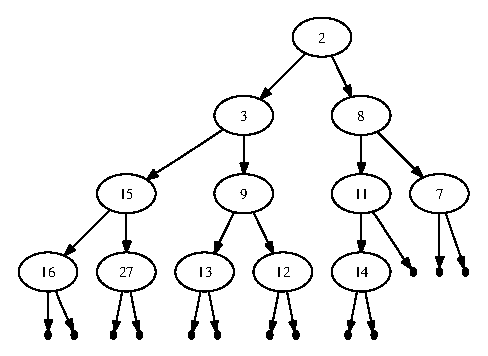
\epsfig{file=nearly-complete-tree.eps}
        \caption{Ein nahezu vollst\"andiger Baum der Tiefe 4.}
        \label{fig:nearly-complete-tree.eps}
      \end{figure}
      
      Stellen wir diesen Baum durch ein Feld dar, so erhalten wir das folgende Feld:
      \\[0.2cm]
      \hspace*{1.3cm}
      \texttt{[ 2, 3, 8, 15, 9, 11, 7, 16, 27, 13, 12, 14]} 
      \\[0.2cm]
      Dieses Feld entsteht aus dem vorigen Feld dadurch, dass wir die letzten drei
      Eintr\"age gel\"oscht haben.  Schlie\3lich zeigt Abbildung
      \ref{fig:not-nearly-complete-tree.eps} auf Seite
      \pageref{fig:not-nearly-complete-tree.eps} noch einen bin\"aren Baum, der nicht nahezu
      vollst\"andig ist, denn er enth\"alt auf der untersten Ebene eine L\"ucke, weil die Knoten
      nicht von rechts nach links entfernt wurden.

      \begin{figure}[!ht]
        \centering
        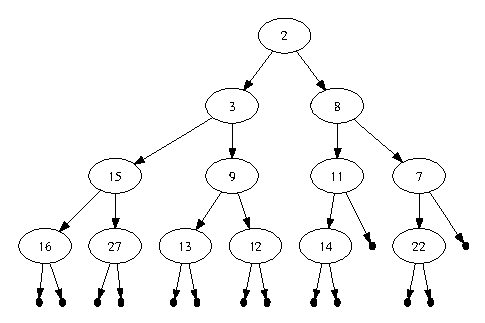
\epsfig{file=not-nearly-complete-tree.eps}
        \caption{Ein Baum, der nicht nahezu vollst\"andig ist.}
        \label{fig:not-nearly-complete-tree.eps}
      \end{figure}

      Bezeichnen wir die Menge der nahezu vollst\"andigen bin\"aren B\"aume mit $\Bin^*$, so
      k\"onnen wir diese Menge formal durch eine Induktion definieren:
      \begin{enumerate}
      \item $n \in \overline{\Bin} \rightarrow n \in \Bin^*$,

            jeder vollst\"andige bin\"are Baum ist nat\"urlich erst recht nahezu vollst\"andig.
      \item $l \in \overline{\Bin} \wedge l.\textsl{height}() = h \wedge r \in \overline{\Bin}
             \wedge r.\textsl{height}() = h-1 \,\rightarrow\,
             \textsl{node}(k,v,l,r) \in \Bin^*$,

            falls $l$ ein vollst\"andiger bin\"arer Baum der H\"ohe $h$ ist und $r$ ein 
            vollst\"andiger bin\"arer Baum der H\"ohe $h-1$, dann ist
            $\textsl{node}(k,v,l,r)$ ein nahezu vollst\"andiger bin\"arer Baum.
      \item $l \in \overline{\Bin} \wedge l.\textsl{height}() = h \wedge r \in \Bin^*
             \wedge r.\textsl{height}() = h \,\rightarrow\,
             \textsl{node}(k,v,l,r) \in \Bin^*$,

            falls $l$ ein vollst\"andiger bin\"arer Baum der H\"ohe $h$ ist und $r$ ein nahezu
            vollst\"andiger bin\"arer Baum, der ebenfalls die H\"ohe $h$ hat, dann ist
            $\textsl{node}(k,v,l,r)$ ein nahezu vollst\"andiger bin\"arer Baum.

      \item $l \in \Bin^* \wedge l.\textsl{height}() = h \wedge r \in \overline{\Bin}
             \wedge r.\textsl{height}() = h-1 \,\rightarrow\,
             \textsl{node}(k,v,l,r) \in \Bin^*$,

            falls $l$ ein nahezu vollst\"andiger bin\"arer Baum der H\"ohe $h$ ist und $r$ ein 
            vollst\"andiger bin\"arer Baum der H\"ohe $h-1$ hat, dann ist
            $\textsl{node}(k,v,l,r)$ ein nahezu vollst\"andiger bin\"arer Baum.
      \end{enumerate}
\end{enumerate}
Nahezu vollst\"andige bin\"are B\"aume lassen sich durch ein Feld darstellen, weil dann f\"ur
den linken und den rechten Teilbaum keine expliziten Referenzen abgespeichert werden
m\"ussen.  Das spart Speicherplatz, die Implementierung ist aber etwas komplizierter als die
von uns entwickelte Variante.

Wir kommen nun zur\"uck zur Diskussion der Klasse \texttt{PriorityQueue}.
Diese Klasse enth\"alt die folgenden Konstruktoren.
\begin{enumerate}
\item \texttt{PriorityQueue()}

      Dieser Konstruktor erzeugt einen neue Priorit\"ats-Warteschlange.
      Das zu Grunde liegende Feld hat dabei zun\"achst die Gr\"o\3e 11.
      Wenn sp\"ater der Platz in diesem Feld nicht mehr ausreicht, wird es dynamisch
      vergr\"o\3ert. 
\item \texttt{PriorityQueue(Collection<E> $c$)}
  
      Dieser Konstruktor erzeugt eine Priorit\"ats-Warteschlange, die alle Elemente der
      Zusammenfassung $c$ enth\"alt.
\item \texttt{PriorityQueue(int initialCapacity)}
  
      Dieser Konstruktor  erzeugt eine neue Priorit\"ats-Warteschlange.
      Das zu Grunde liegende Feld hat dabei die Gr\"o\3e \texttt{initialCapacity}.
\item \texttt{PriorityQueue(int initialCapacity, Comparator<E> comparator)}

      Dieser Konstruktor  erzeugt einen neue Priorit\"ats-Warteschlange.
      Das zu Grunde liegende Feld hat dabei die Gr\"o\3e \texttt{initialCapacity}.
      Die Elemente dieser Warteschlange werden nicht durch einen Aufruf der
      Methode 
      \\[0.2cm]
      \hspace*{1.3cm}
      $x.\texttt{compareTo}(y)$ 
      \\[0.2cm]
      verglichen, sondern statt dessen wird der als Argument \"ubergebene Comparator
      zum Vergleich benutzt:
      \\[0.2cm]
      \hspace*{1.3cm}
      $\mathtt{comparator}.\texttt{compare}(x,y)$. 
\end{enumerate}
Die Methoden, die zur Verf\"ugung gestellt werden, kennen wir schon aus unserer Diskussion
der Schnittstellen \texttt{Collection<E>} und \texttt{Queue<E>}. 
\begin{enumerate}
\item \texttt{boolean offer(E $e$)}

      Der Aufruf $q.\mathtt{offer}(e)$ f\"ugt das Element $e$ in die
      Priorit\"ats-Warteschlange $q$ an und
      entspricht unserer Methode \textsl{insert}. 
\item \texttt{E peek()}

      Der Aufruf $q.\mathtt{peek}()$ liefert das Element mit der h\"ochsten Priorit\"at in der
      Priorit\"ats-Warte\-schlange $q$ als Ergebnis.   $q$ wird dabei nicht ver\"andert.  Falls $q$
      leer ist, wird \texttt{null} zur\"uck gegeben.
\item \texttt{E poll()}

      Der Aufruf $q.\mathtt{poll}()$ liefert das Element mit der h\"ochsten Priorit\"at in der
      Priorit\"ats-Warte\-schlange $q$ als Ergebnis.  
      Das Element wird dabei aus $q$ entfernt.  Falls $q$
      leer ist, wird \texttt{null} zur\"uck gegeben.
\item \texttt{boolean remove(E $e$)}

      Der Aufruf $q.\mathtt{remove}(e)$ entfernt das Element $e$ aus
      der Priorit\"ats-Warteschlange $q$.  Falls $q$ das Element $e$ nicht enth\"alt, bleibt
      $q$ unver\"andert.  In diesem Fall wird als Ergebnis \texttt{false} zur\"uck gegeben,
      sonst wird \texttt{true} zur\"uck gegeben.
\end{enumerate}
Die Klasse \texttt{PriorityQueue} enth\"alt keine Methode, um die Priorit\"at eines Elements
zu \"andern.  Das geht auch gar nicht, denn bei dieser Klasse wird nicht zwischen dem Wert
und dem Schl\"ussel unterschieden, beide sind Teil eines Elements.  Um also einen Priorit\"at
zu \"andern, m\"ussen wir das betreffende Element zun\"achst aus der Priorit\"ats-Warteschlange
entfernen, die Priorit\"at \"andern und anschlie\3end das Element mit der ge\"anderten Priorit\"at
wieder einf\"ugen.


%\subsection{Repr\"asentierung von Heaps durch Listen}
Anstatt  Heaps durch bin\"are B\"aume zu repr\"asentieren, k\"onnen wir Heaps auch
durch Listen darstellen.   Die Idee ist, einen Heap durch eine  Liste der Form \\[0.1cm]
\hspace*{1.3cm} 
$L = \bigl[ \pair(k_1,v_1), \pair(k_2,v_2), \pair(k_3,v_3), \cdots, \pair(k_n,v_n) \bigr]$
\\[0.1cm]
zu repr\"asentieren.  Dazu m\"ussen wir zun\"achst festlegen, wie eine solche Liste als Heap
interpretiert werden kann.  Wir definieren daher eine Funktion \\[0.1cm]
\hspace*{1.3cm} 
$\textsl{interpret}: \textsl{List}\bigl((\textsl{Key}\times \textsl{Value})\cup \{\Omega\}\bigr) \times \mathbb{N}  \rightarrow \textsl{Heap}$
\\[0.1cm]
die eine Liste, deren Elemente entweder Paare von Priorit\"aten und Werten sind, oder aber
der spezielle Wert $\Omega$, in einem Heap umwandelt.  Die Funktion \textsl{interpret}
bekommt als zweites Argument einen Index, der in die Liste zeigt. Die Idee ist, dass der
Wert, der in der Liste unter diesem Index abgespeichert ist, die Wurzel des Baums
$\textsl{interpret}(L,i)$ markiert.  Bei der Definition von \textsl{interpret} gibt es zwei
F\"alle:
\begin{enumerate}
\item $L(i) = \Omega$.  Dann gilt nat\"urlich \ 
       $\textsl{interpret}(L,i) = \textsl{nil}$.
\item $L(i) = \pair(k, v)$. Dann gilt:\\[0.1cm]
      \hspace*{1.3cm} 
      $\textsl{interpret}(L,i) = \textsl{node}\bigl(k,v,\textsl{interpret}(L,2*i),\textsl{interpret}(L,2*i+1)\bigr)$.

      Die Idee bei dieser Definition ist es, dass der linke Sohn des durch den Index $i$
      repr\"asentierten Knotens an der Stelle $2*i$ abgespeichert wird, w\"ahrend der rechte
      Sohn unter dem Index $2*i + 1$ abgespeichert wird.
\end{enumerate}
Abbildung \ref{fig:heap-list} auf Seite \pageref{fig:heap-list} zeigt einen Heap, der die Zahlen $1, \cdots, 9$ als
Priorit\"aten enth\"alt.  Als Werte sind die Buchstaben ``\texttt{a}'', $\cdots$,
``\texttt{i}'' eingetragen.
  Als Liste repr\"asentiert hat dieser Heap die Form \\[0.1cm]
\hspace*{1.3cm} $L = \bigl[ \pair(1,\mathtt{a}), \pair(2,\mathtt{b}),
\pair(3,\mathtt{c}), \pair(4,\mathtt{d}), \pair(6,\mathtt{f}), 
\pair(5,\mathtt{e}), \pair(7,\mathtt{g}), \pair(8,\mathtt{h}), \Omega, \Omega,
\Omega, \pair(9, \mathtt{i}) \bigr]$.
\\[0.1cm]
Diese Liste hat gewissermassen L\"ocher, die durch die drei $\Omega$s repr\"asentiert
werden. Diese $\Omega$s entsprechen dem rechten Teilbaum des mit $4$ beschrifteten Knotens
und die beiden Teilb\"aume des mit $6$ beschrifteten Knotens.
Wollen wir Heaps durch Listen auf die oben skizzierte Weise implementieren, so brauchen wir au\3er der Liste $L$ noch
eine Liste \textsl{Counts}, wobei $\textsl{Counts}(i)$ die Zahl der Knoten in dem Teilbaum
angibt, dessen Wurzel an der Stelle $i$ in der Liste $L$ steht. 
Schlie\3lich ben\"otigen wir zur effizienten Implementierung der Methode $\textsl{change}()$
noch eine Funktion, die zu einem gegebenen Wert $v$ den Index $i$ berechnet, f\"ur den 
 $L(i) = \pair(k,v)$ \\[0.1cm]
gilt.  Wir realisieren diese Funktion in Form einer bin\"aren Relation.  Diese bin\"are
Relation speichern wir in der Instanz-Variablen \texttt{nodeIndex} ab.
Das folgende Listing zeigt die Listen-basierte Implementierung der Klasse \textsl{Heap}.

\begin{Verbatim}[ frame         = lines, 
                  framesep      = 0.3cm, 
                  labelposition = bottomline,
                  numbers       = left,
                  numbersep     = -0.2cm,
                  xleftmargin   = 0.8cm,
                  xrightmargin  = 0.8cm
                ]
    class body Heap;
   
        var L;
        var Counts;
        var nodeIndex;
   
        procedure create();
            L      := [];
            Counts := [];
            nodeIndex := {};
        end create;
   
        procedure insert(k, v);
            insertIndex(k, v, 1);
        end insert;
   
        procedure insertIndex(k, v, idx);
            if L(idx) = om then
                L(idx) := [ k, v ];
                Counts(idx) := 1;
                Counts(2 * idx) := 0;
                Counts(2 * idx + 1) := 0;
                nodeIndex(v) := idx;
                return;
            end if;
            Counts(idx) +:= 1;
            [ k1, v1 ] := L(idx);
            if k1 <= k then
                if Counts(2 * idx + 1) < Counts(2 * idx) then
                    insertIndex(k, v, 2 * idx + 1);
                else 
                    insertIndex(k, v, 2 * idx);
                end if;
                return;
            end if;
            L(idx) := [k, v];
            nodeIndex(v)  := idx;
            nodeIndex(v1) := om;
            if Counts(2 * idx + 1) < Counts(2 * idx) then
                insertIndex(k1, v1, 2 * idx + 1);
            else
                insertIndex(k1, v1, 2 * idx);
            end if;
        end insertIndex;
   
        procedure change(v, k);
            idx := nodeIndex(v);
            if idx = 1 then
                L(1) := [k, v];
            else
                parentIdx := idx / 2;
                [ kp, vp ] := L(parentIdx);
                if k < kp then
                    L(idx)       := [ kp, vp ];
                    L(parentIdx) := [ k, v ];
                    nodeIndex(vp) := idx;
                    nodeIndex(v)  := parentIdx;
                    change(v, k);
                else 
                    L(idx) := [ k, v ];
                end if;
            end if;
        end change;
   
        procedure top();
            return L(1);
        end top;
   
        procedure remove();
            removeIndex(1);
        end remove;
   
        procedure removeIndex(idx);
            if L(idx) = om then
                return;
            end if;
            Counts(idx) -:= 1;
            [k, v] := L(idx);
            nodeIndex(v) := om;
            if L(2 * idx) = om and L(2 * idx + 1) = om then
                L(idx) := om;
                Counts(2 * idx) := om;
                Counts(2 * idx + 1) := om;
                return;
            end if;
            if L(2 * idx) /= om and L(2 * idx + 1) = om then
                [k1, v1] := L(2 * idx);
                L(idx) := L(2 * idx);
                removeIndex(2 * idx);
                nodeIndex(v1) := idx;
                return;
            end if;
            if L(2 * idx) = om and L(2 * idx + 1) /= om then
                [k2, v2] := L(2 * idx + 1);
                L(idx) := L(2 * idx + 1);
                removeIndex(2 * idx + 1);
                nodeIndex(v2) := idx;
                return;
            end if;
            [ k1, v1 ] := L(2 * idx);
            [ k2, v2 ] := L(2 * idx + 1);
            if k1 <= k2 then
                L(idx) := [ k1, v1 ];
                removeIndex(2 * idx);
                nodeIndex(v1) := idx;
            else
                L(idx) := [ k2, v2 ];
                removeIndex(2 * idx + 1);
                nodeIndex(v2) := idx;
            end if;
        end removeIndex;
   
        procedure isEmpty();
            return L(1) = om;
        end isEmpty;
   
    end Heap;
\end{Verbatim}

%%% Local Variables: 
%%% mode: latex
%%% TeX-master: "algorithmen"
%%% End: 


%%% Local Variables: 
%%% mode: latex
%%% TeX-master: "algorithmen"
%%% End: 
